
\chapter{Estado del Arte}
    Organización: 
        - Presentar el problema que estamos resolviendo.
        - Consultar artículos en los últimos años realcionados con el problema
        - Como no hay muchos artículos recurir a técnicas de Deep Learning de reconocimiento de Landmarks 
        - Explicar qué se hace en este campo y por qué elegimos 3FabRec

    \noindent En esta sección nuestro objetivo será realizar una investigación por la literatura y los artículos publicados relacionados con el campo de invesitgación del reconocimiento automático de landmarks cefalométricos en tareas de antropología forense. Para ello utilizaremos la base de datos \textit{Scopus} para realizar la búsqueda y consulta de artículos científico publicados.

    \section{Localización de landmarks cefalométricos en imágenes}
        \subsection{Soluciones clásicas}

        \subsection{Métodos actuales}
            \noindent Actualmente este campo de investigación se encuentra aún en vías de desarrollo, aunque bien es cierto que con el interés creciente en el \textit{Deep Learning} se están comenzando a ver nuevas publicaciones con métodos basados en redes neuronales convolucionales que obtienen buenos resultados. 

            \medskip

            \noindent Para hacernos una primera idea del estado actual del problema de reconocimiento de landmarks faciales en imágenes realizamos una primera consulta en \textit{SCOPUS} \autoref{fig:SCOPUS1} con la siguiente \textit{keyword} restringiendo los artículos a aquellos relacionados con la informática:
            
            \begin{verbatim}
                TITLE-ABS-KEY ( 
                    facial  
                    AND  
                    ( landmarks  OR  keypoints )  
                    AND  
                    detection 
                    )  
                    AND  
                    ( LIMIT-TO ( SUBJAREA ,  "COMP" ) )
            \end{verbatim}
            
            \medskip
            
            \noindent Como podemos observar, actualmente existe una tendencia creciente en la publicación de papers relacionados con este tema, en particular esta tendencia comienza en los años en que surge el Deep Learning y las CNN comienzan a utilizarse en visión por computador para el tratamiento de imágenes. 

            \begin{figure}[!h]
                \centering
                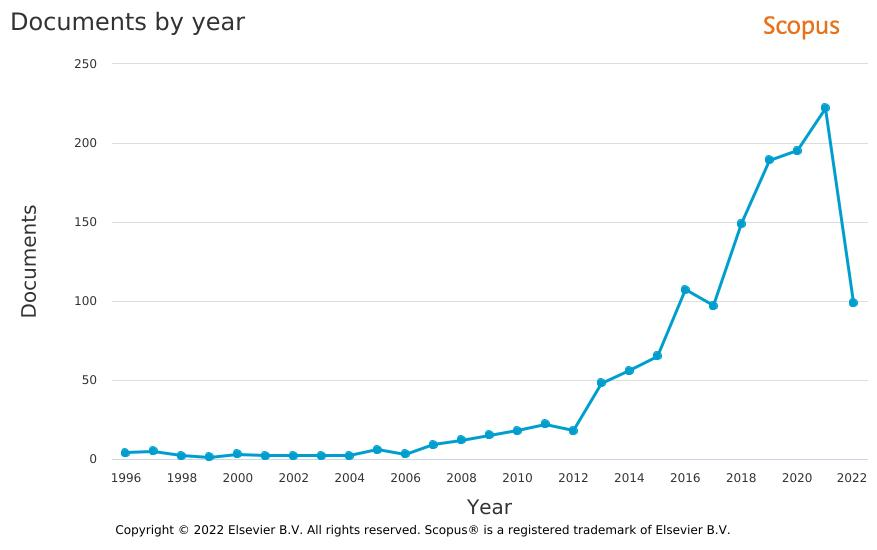
\includegraphics[width=0.6\textwidth]{img/Scopus_1.jpg}
                \caption{Gráfica de publicaciones por año obtenida con la primera \textit{keyword}. Destaca el notable incremento de papers a partir de 2012, año en que aparece la red AlexNet y comienza a ganar popularidad el Deep Learning en el tratamiento de imágenes.}
                \label{fig:SCOPUS1}
            \end{figure}

            \medskip

            \noindent Sin embargo los artículos que se han encontrado en \autoref{fig:SCOPUS1} no guardan una relación muy estrecha con el problema de deteción de landmarks cefalométricos en problemas de antropología forense, por ello para descubrir el estado del arte en este campo nos vemos obligados a realizar otra consulta en scopus un poco más concreta y que nos permita conocer mejor las publicaciones más relevantes en este campo en los últimos años descartando los que no sean artículos relacionados con informática. La consulta que realizamos es la siguiente: 

            \begin{verbatim}
                TITLE-ABS-KEY ( 
                    ( 
                        ( anthropology  OR  ( anthropology  AND  forensic ) )  
                        AND  
                        ( cephalometric  AND  ( landmarks  OR  keypoints ) ) 
                    )  
                    
                    OR  
                    
                    ( 
                        ( anthropology  OR  ( anthropology  AND  forensic ) )  
                        AND  
                        ( facial  AND  ( landmarks  OR  keypoints ) ) 
                    ) 
                    )  
                    AND  
                    ( LIMIT-TO ( SUBJAREA ,  "COMP" ) )
            \end{verbatim}

            \medskip

            \noindent Con la búsqueda anterior se obtienen un total de $14$ artículos, algo que nos confirma que se encuentra de un campo de investigación en vías de desarrollo con apenas bibliografía. Podemos ver un gráfico de resultados de la búsqueda en \autoref{fig:SCOPUS2}.

            \begin{figure}[!h]
                \centering
                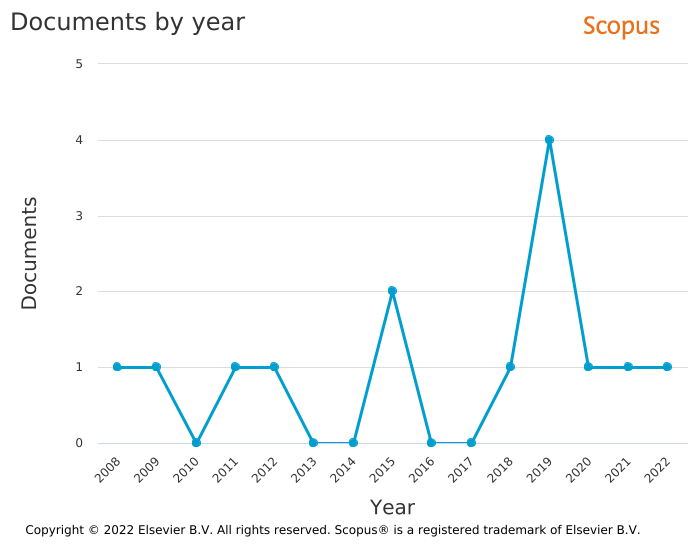
\includegraphics[width=0.8\textwidth]{img/Scopus_2.png}
                \caption{Gráfica de publicaciones por año obtenida con la segunda \textit{keyword}. La tendencia es a un artículo por año, aunque destaca el pico de tres artículos en 2015 y el de cuatro en 2019.}
                \label{fig:SCOPUS2}
            \end{figure}

            \medskip

            \noindent De los catorce artículos vamos a destacar los siguientes por la relación directa con nuestro problema ordenados de mayor a menor antigüedad: 

            \subsubsection{Two different approaches to handle landmark location uncertainty in skull-face overlay: coevolution vs fuzzy landmarks}
                \noindent Se trata de un artículo pulicado en $2011$ por Óscar Ibáñez, Óscar Cordón y Sergio Damas \cite{ibanez2011two} en el cual abordan el problema de la superposición craneofacial diseñando un nuevo algoritmo basado en coevolución capaz de reducir el proceso de \textit{Skull-face overlay} (SFO) que tradicionalmente podía llegar a tardar unas 24 horas y comparándolo con un algoritmo ya existente basado en landmarks imprecisos en el cual el antropólogo forense marca regiones de la imagen en las que se encuentra cada landmark (esta tarea no está automatizada en este algoritmo).

                \medskip

                \noindent Durante el proceso de SFO se dispone de un modelo $3$D de un cráneo y de una imagen, de manera que se considera exitoso el proceso cuando se coloca el cráneo en la misma posición en que aparece en la imagen. Durante este proceso se deben tener en cuenta factores como la edad de la persona, el peso o las expresiones faciales, que añaden un grado más de dificultad a la tarea.

                \medskip

                \noindent Generalmente se dispone de un conjunto de landmarks marcados tanto en la imagen como en el cráneo, y la tarea del SFO se reduce en calcular la transformación que permite llevar los landmarks del cráneo a ocupar la misma posición que en la imagen.

                \medskip

                \noindent La alternativa al algoritmo basado en landmarks imprecisos es un algorimto coevolutivo en el cual el valor de la función de fitness de cada elemento depende de la de él mismo y otros individuos que pueden interaccionar de forma cooperativa o conflictiva. Adaptado al problema de SFO tendríamos dos poblaciones: el conjunto de parámetros que definen la transformación que se aplica al modelo $3$D del cráneo y por otro lado las localizaciones de los landmarks cefalométricos. Ambas poblaciones colaboran para encontrar la mejor transformación posible y solucionar el SFO.

                \medskip

                \noindent En el experimento se disponía de seis procesos distintos de SFO correspondientes a tres casos reales proporcionados por el laboratorio de Antropología Física de la Universidad de Granada en colaboración con la policía científica. Se disponía así de tres modelos $3$D de cráneos pertenecientes a personas desaparecidas junto con un dataset de seis imágenes. Las imágenes, a pesar de ser pocas, presentan una gran variedad en iluminación, posición (hay imágenes frontales y en $3/4$) y con problemas de oclusión en algunos casos para los landmarks a causa del cabello. Por otro lado la calidad de las imágenes es muy variada, habiendo imágenes de gran resolución y otras de baja calidad. Finalmente se disponen cuatro imágenes para el caso de estudio $3$ y una única imagen para el caso de estudio $1$ y $2$.

                \medskip
                

                \noindent En el experimento, el algoritmo empleado para la técnica de encontrar landmarks imprecisos es CMA-ES, y se comparó con el algoritmo coevolutivo desarrollado. Las conclusiones fueron que el nuevo algoritmo reducía considerablemente los tiempos de ejecución del algoritmo basado en landmarks imprecisos y que realizaba una Localización de landmarks cefalométricos apropiada. 
                
                \medskip

                \noindent Por lo tanto podemos considerar este primer algorimto coevolutivo como la primera aproximación a nuestro problema de detección automática de landmarks.

            \subsubsection{Automatic craniofacial anthropometry landmarks detection and measurements for the orbital region}
                \noindent Se trata de un artículo publicado en $2014$ por Salina Mohd, Nor Hidayah, Roshahida Ahmad, Effirul Ikhwan y Zainal Arif \cite{asi2014automatic}








\endinput
%------------------------------------------------------------------------------------
% FIN DEL CAPÍTULO. 
%------------------------------------------------------------------------------------

